Электромагнитная волна --- синусоидальное электромагтиное колебание в пространстве~\cite{meanders:radiovolny}. Другими словами, ЭМВ --- это направленный поток фотонов. Источником радиоволны может быть любой электрический проводник, в котором движется переменный электрический ток. Электромагнитная волна состоит из электрического и магнитного синусоидального колебания, ориентированных друг относительно друга перпендикулярно (рисунок~\ref{fig:emf}).

\begin{figure}[ht]
    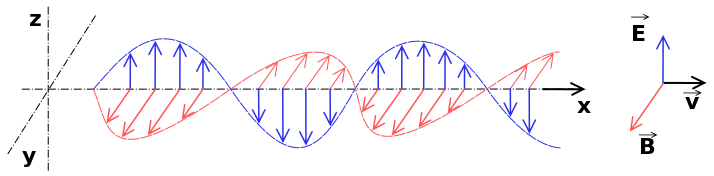
\includegraphics[width=.8\linewidth]{Figures/emf.png}
    \caption{Электромагнитная волна}
    \label{fig:emf}
\end{figure}

Радиоволны --- электромагнитное излучение с длинами волн в электромагнитном спектре длиннее инфракрасного света~\cite{wiki:radiowaves}. Радиоволны имеют частоту от 3 кГц до 300 ГГц, и соответствующую длину волны от 1 миллиметра до 100 километров. Естественными источниками радиоволн являются молнии и астрономические объекты. Искусственно созданные радиоволны используются для стационарной и мобильной радиосвязи, радиовещания, радиолокации и других навигационных систем, спутников связи, компьютерных сетей и других бесчисленных приложений. Различные частоты радиоволн по-разному распространяются в атмосфере Земли: длинные волны могут покрыть часть Земли очень последовательно, более короткие волны могут отражаться от ионосферы и распространяются по всему миру, и с еще более короткими длинами радиоволны изгибаются или отражаются очень слабо и распространяются в пределах прямой видимости.

Земная атмосфера прозрачна почти полностью для падающего извне излучения лишь в двух сравнительно узких окнах: оптическом --- в диапазоне длин волн $\lambda$ от 0.3 мкм до 2 мкм (область до 8 мкм состоит из ряда узких полос пропускания) и в радиодиапазоне --- для волн длиной от 1 мм до 30 м~\cite{astronet:atmosphere}. Непрозрачность атмосферы для всех др. длин волн определяется поглощением и рассеянием излучения на молекулах и атомах, а также отражением радиоволн от электронов ионосферы (рисунок~\ref{fig:atmosphere}~\cite{wiki:radiowaves}).

\begin{figure}[ht]
    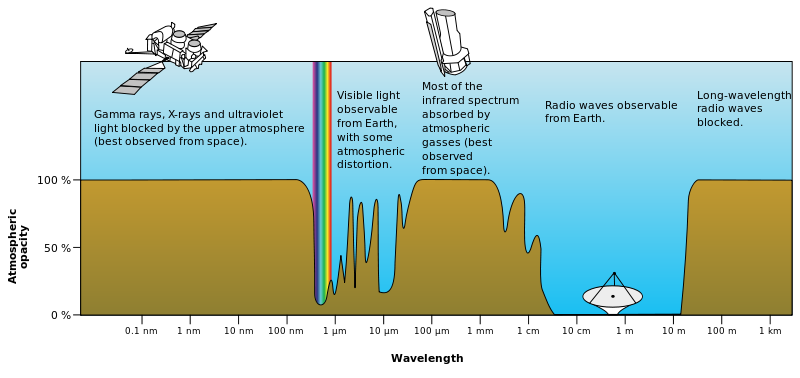
\includegraphics[width=1\linewidth]{Figures/radiowaves.png}
    \caption{Непрозначность атмосферы Земли для различных длин волн электромагнитного излучения, включая радиоволны}
    \label{fig:atmosphere}
\end{figure}

Электромагнитные волны (радиоволны) распространяются в вакууме со скоростью света --- 299, 792, 458 м/с.

Частота колебаний выражается через длину волны (формула~\eqref{eq:lambda}):

\begin{equation}
    \label{eq:lambda}
    f = \frac{c}{\lambda},
\end{equation}

где f --- частота, $\lambda$ --- длина волны, c --- скорость света.

Радиоволны подразделяются на несколько диапазонов (таблица~\ref{tab:radiorange}):

\begin{longtable}[c]{|c|c|c|}
    \caption{Диапазон радиоволн}
    \label{tab:radiorange}\\
    \hline
    \textbf{Диапазон} & \textbf{Частота} & \textbf{Длина волны}\\
    \hline
    \endfirsthead
    \hline
    \textbf{Диапазон} & \textbf{Частота} & \textbf{Длина волны}\\
    \hline
    \endhead
        Сверхдлинные <<СДВ>> & 3 -- 30 кГц & 100 -- 10 км\\
        \hline
        Длинные <<ДВ>> & 30 -- 300 кГц & 10 -- 1 км\\
        \hline
        Средние <<СВ>> & 300 -- 3000 кГц & 1000 -- 100 м\\
        \hline
        Короткие <<КВ>> & 3 -- 30 МГц & 100 -- 10 м\\
        \hline
        Ультракороткие <<УКВ>> & 30 МГц -- 6000 ГГц & 10 м -- 0.05 мм\\
        \hline
\end{longtable}

Ультракороткие, в свою очередь, включают (таблица~\ref{tab:ultrarange}):

\begin{longtable}[c]{|c|c|c|}
    \caption{Ультракороткие радиоволны}
    \label{tab:ultrarange}\\
    \hline
    \textbf{Диапазон} & \textbf{Частота} & \textbf{Длина волны}\\
    \hline
    \endfirsthead
    \hline
    \textbf{Диапазон} & \textbf{Частота} & \textbf{Длина волны}\\
    \hline
    \endhead
        Метровые <<МВ>> & 30 -- 300 МГц & 10 -- 1 м\\
        \hline
        Дециметровые <<ДМВ>> & 300 -- 3000 МГц & 10 -- 1 дм\\
        \hline
        Сантиметровые <<СМВ>> & 3 -- 30 ГГц & 10 -- 1 см\\
        \hline
        Миллиметровые <<ММВ>> & 30 -- 300 ГГц & 10 -- 1 мм\\
        \hline
        Субмиллиметровые <<СММВ>> & 300 -- 6000 ГГц & 1 -- 0.05 мм\\
        \hline
\end{longtable}

Диапазоны от дециметровых до миллиметровых волн, из-за их очень высокой частоты, называют сверхвысокими частотами <<СВЧ>>.

Распространение волны ограничивается её длиной: чем выше длина волны (меньше частота), тем она более способна огибать препятствия.
